\documentclass[a4,12pt,footinclude=true,oneside,headinclude=true]{scrartcl} %Need KOMA
\usepackage{cookby}

% Customize your cookbook to your preferred language. Default is german. 
\usepackage[ngerman]{babel} % change language, e.g. to english

% What is the term: "Recipes" in your native language? 
\RecipesinLanguage{Rezepte}

%What is the term: "Cookbook" in your native language?
\CookbookinLanguage{Rezeptebuch}

%What is the term: "page" (of a book) in your native language?
\PageinLanguage{Seite}
%What is the term: "version" in your native language? (Leave a blank space after the word)
\VersioninLanguage{Stand}	

%What is the term: "minutes" (plural) in your native language?
\MinutesinLanguage{Minuten}

%What is the term: "hours" (plural) in your native language?
\HoursinLanguage{Stunden}

% Where to download the newest version of your cookbook?
\website{https://github.com/jokobus/cookby} 
% This does not work: example.com
% This works: www.example.com or https://example.com

% Which color shall the comments have?
\CommentColor{gray}

% Your name 
% emailadress (without mailto:...) is optional
\author[myemail@cookby.com]{Jokobus}

% Default baking instruction for the oven (e.g. w/ w/o circulation fan?)
\DefaultBakingSettings{Umluft}

\begin{document}

	\begin{titlepage}
		\maketitle
		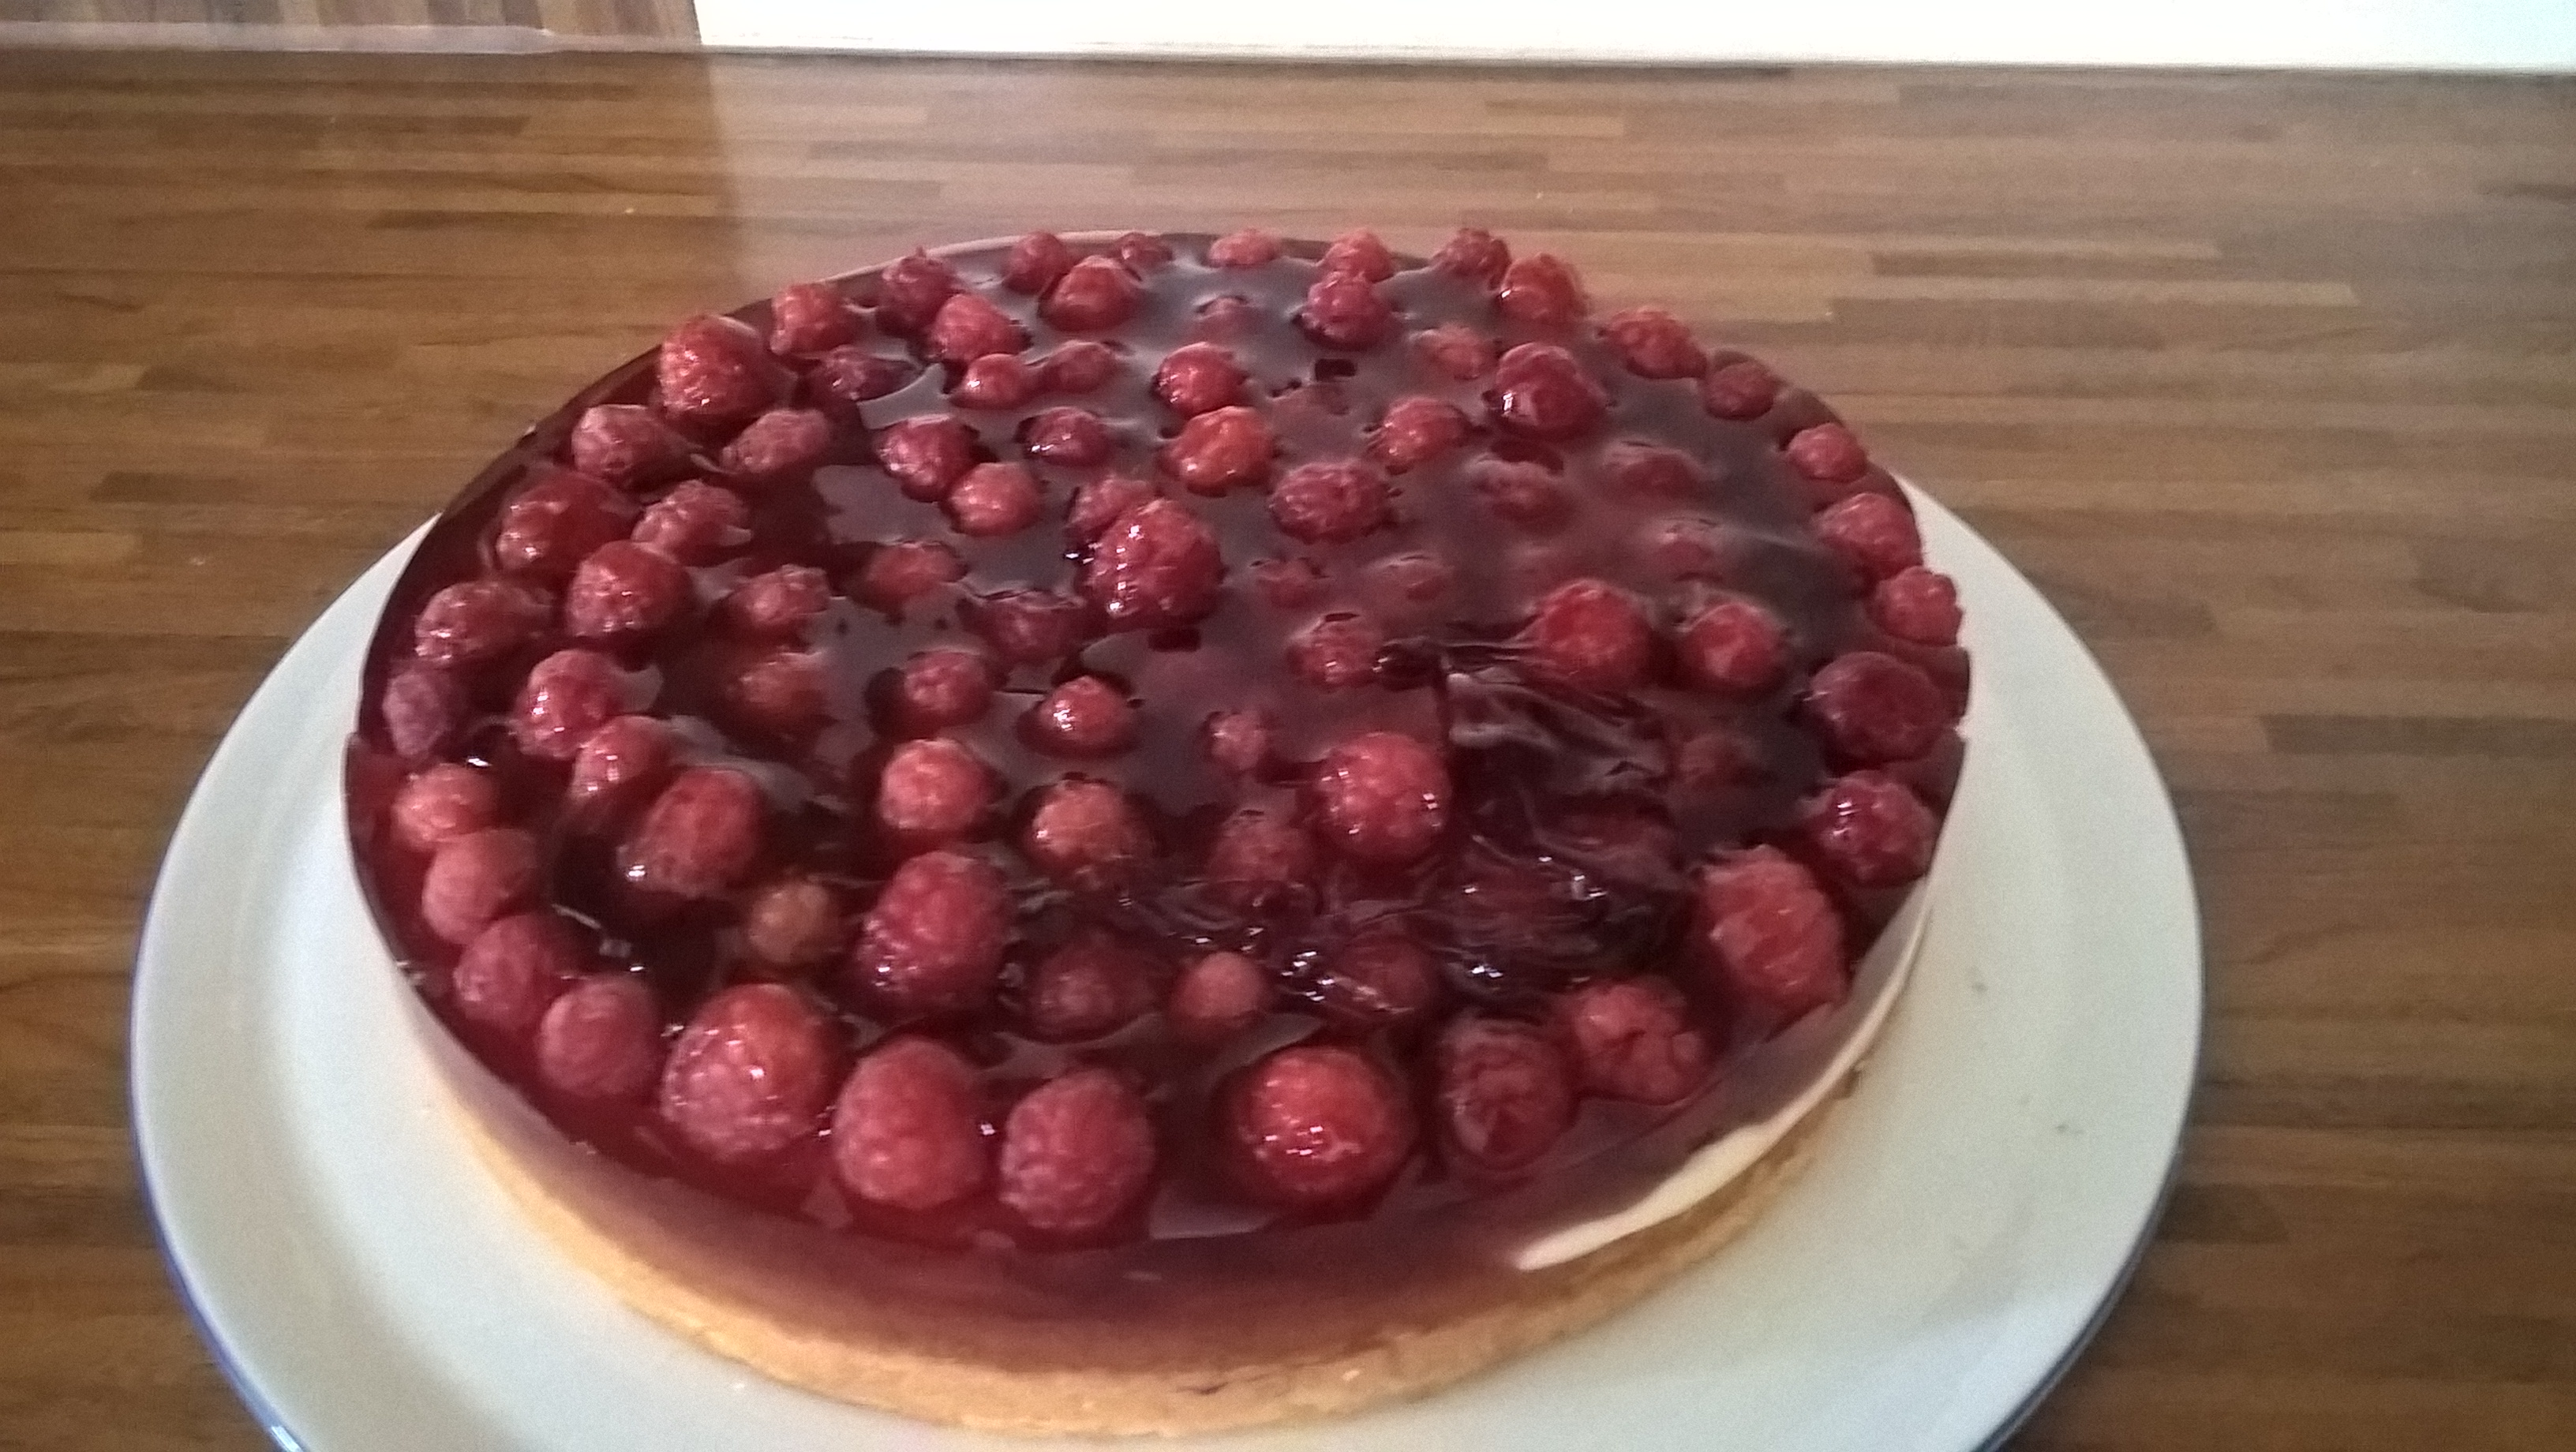
\includegraphics[width=\textwidth]{cake.jpg}
		\thispagestyle{empty}
	\end{titlepage}
	
	% Build the table of contents
	{\setcounter{page}{2}
		\normalfont
		%\label{HereIsTheTableOfContent}
		\tableofcontents
		\pagebreak
	}
	
\section{Nussecken}

\smallcomment{Perfekt zum Verschenken!}


Teig: 
\begin{ingredients}
	\item 300g Mehl
	\item 1 gehäufter TL Backpulver 
	\item 150g Butter und oder Margarine
	\item 120g Zucker (und Puderzucker)
	\item 5 Päckchen Vanillezucker
	\item 2 Eier 
	\item 4 -- 6 Tropfen Butter-Vanille-Backaroma
	\subitem zu einem glatten, straffen Teig verkneten
\end{ingredients}
	Nussmasse: 

\begin{ingredients}
	\item 200g -- 250g Butter oder Margarine
	\item 200g Zucker
	\item 5 EL Sahne 
		\subitem kurz aufkochen
	\item 500g gemahlene Nüsse ($\nicefrac{1}{2}$ davon nur grob)
		\subitem einrühren, etwas abkühlen
	\item 4 -- 6 Tropfen Bittermandelaroma
		\subitem dazu, Teig auf das Blech ausrollen, mit
	\item ca. 10 EL Marmelade (Aprikosen- und Orangenmarmelade)
		\subitem bestreichen, Nussmasse gleichmäßig verteilen, etwas andrücken, mit
	\item Rum-, Bittermandel- und Vanillearoma
		\subitem aromatisieren bzw. abschmecken
\end{ingredients} 
\baking{170}{20--30}

\begin{comment}
	\citem Noch warm in Ecken schneiden 
	\citem Mit Kuvertüre garnieren
\end{comment}
\pagebreak


\section{Rohrnudeln}
	\begin{ingredients} 
		\item 500g Mehl
		\item 1 Päckchen Trockenhefe / 1 Würfel frische Hefe
		\item 225ml lauwarme Milch
		\item 80g weiche Butter
		\item 60g Zucker
		\item 1 Ei
		\item 1 Prise Salz
			\subitem Alle Zutaten in eine große Schüssel geben
	\end{ingredients}

	% Discover the commands \prewaiting, \waiting, \prebaking and \baking 
	% prewaiting and prebacking are in the vertical center of the page, waiting and baking are aligned to the bottom of the page
	\prewaiting{15}[Minuten]{zugedeckt ruhen lassen}[Durchkneten bis ein glatter Teig entsteht]
	\prewaiting{1}[Stunde]{zugedeckt ruhen lassen}[Zu Kugeln formen, in Reine setzen, auf jede Kugel ein Stück Butter und etwas Zucker geben]
		
	\baking[]{180}[]{Ca. 30}[Goldgelb backen]
	\pagebreak 

\end{document}